\documentclass{article}
\usepackage[margin=1.5cm,bottom=2cm]{geometry}
\usepackage{fancyhdr}
\usepackage{graphicx}
\usepackage{amsmath}
\usepackage[export]{adjustbox}
\pagestyle{fancy}

\begin{document}
\fancyhead[L]{ 
\includegraphics[width=2cm]{au_logo.png} }
\fancyhead[R]{CPSC 2320: Computational Physics}
\fancyfoot[C]{\thepage}
\vspace*{0cm}
\begin{center}
	{\LARGE \textbf{Lab 2}}\\
	\vspace{0.25cm}
	{\Large Due: Tuesday, September 22}
\end{center}

\section{Tension in a cable}
A block of mass M is held motionless on a frictionless inclined plane by the means of a string attached to the vertical wall (the string is parallel to the plane).  The mass of the object is 10 kg.  Calculate the tension in the rope for angles between 0$^\circ$ and 90$^\circ$ in 5$^\circ$ increments.
\begin{figure}[ht!]
	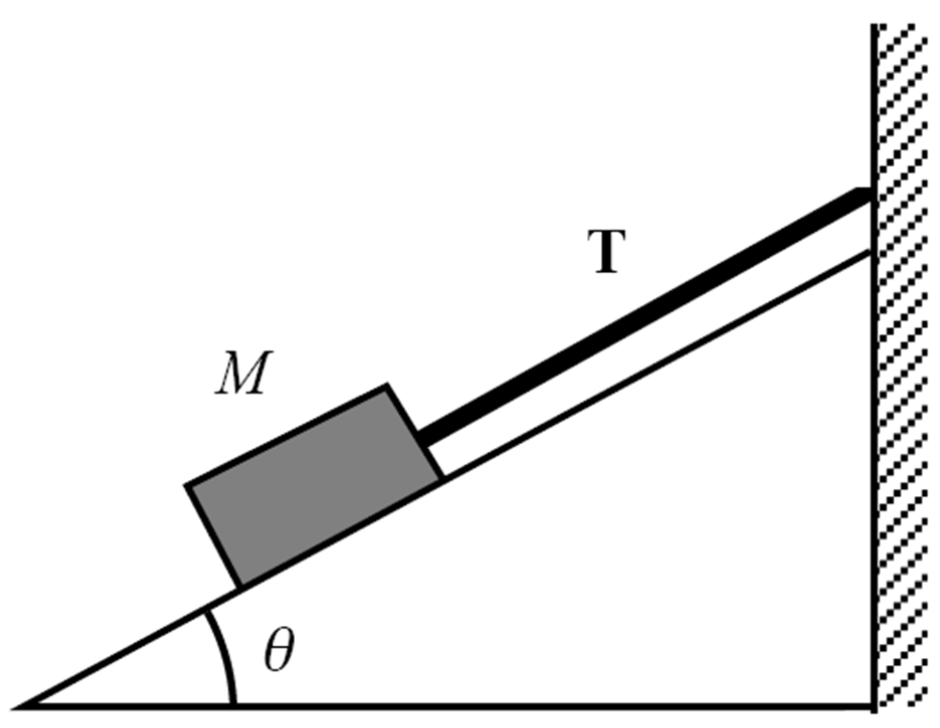
\includegraphics[width=0.4\textwidth,right]{tension.png}
\end{figure}

The equation giving the tension in the rope is:
\begin{equation*}
T=Mg\sin{\theta}
\end{equation*}

Write a C++ function which accepts $M$ and $\theta$ and returns $T$. Declare $g$ as a constant global variable. Use a loop to iterate over $\theta$ and print the tension for each value of $\theta$. Your loop should depend upon variables for the starting, stopping, and increment value of theta (i.e. don't hard code these into your loop).

\section{Max Value of a function}
Consider the function
\begin{equation*}
f(x) = 3x^3+x^2-2x+1
\end{equation*}
We wish to calculate the maximum of this function over the range $x\in(-2,2)$.
Write a C++ program which calculates and stores in an array the values of $f(x)$ over the interval (-2,2) in step sizes of at most $\Delta x$ = 0.1. After filling the array, you should determine the maximum value of the array. Print this value to the user.


\end{document}